\documentclass[11pt]{article}
\usepackage[utf8]{inputenc}
\usepackage[T1]{fontenc}
\usepackage[a4paper,margin=1in]{geometry}
\usepackage{lmodern}
\usepackage{microtype}
\usepackage{amsmath,amssymb,mathtools}
\usepackage{mathrsfs}
\usepackage{tikz-cd}
\usetikzlibrary{arrows}
\usepackage{enumitem}
\usepackage{longtable,booktabs,array}
\usepackage[hidelinks]{hyperref}
\setlength{\parindent}{0pt}
\setlength{\parskip}{0.55em}
\emergencystretch=3em
\hbadness=10000
\hfuzz=20pt
\usepackage[normalem]{ulem}
\newcommand{\K}{K}
\newcommand{\Gr}{\operatorname{Gr}}
\newcommand{\Fil}{\operatorname{Fil}}
\newcommand{\ch}{\operatorname{ch}}
\newcommand{\Todd}{\operatorname{Todd}}
\newcommand{\cl}{\operatorname{cl}}
\newcommand{\Parf}{\operatorname{Parf}}
\newcommand{\Tor}{\operatorname{Tor}}
\newcommand{\Spec}{\operatorname{Spec}}
\newcommand{\RRR}{\mathrm{RRR}}
\providecommand{\codim}{\operatorname{codim}}
\providecommand{\Inv}{\operatorname{Inv}}
\providecommand{\Pic}{\operatorname{Pic}}
\providecommand{\Z}{\mathbb Z}
\providecommand{\Q}{\mathbb Q}
\providecommand{\Ahat}{\widehat A}
\providecommand{\Ahp}{\widehat A^{+}}
\providecommand{\That}{\widehat T}
\providecommand{\rad}{\operatorname{rad}}
\providecommand{\Gl}{\operatorname{Gl}}
\providecommand{\GL}{\operatorname{Gl}}
\providecommand{\ch}{\operatorname{ch}}
\providecommand{\Todd}{\operatorname{Todd}}
\providecommand{\Gr}{\operatorname{Gr}}
\providecommand{\red}{\text{réd}}

% Core macro additions
\providecommand{\Atil}{\widetilde A}
\providecommand{\Ctil}{\widetilde C}
\providecommand{\K}{\mathrm K}
\providecommand{\cC}{\mathcal C}
\providecommand{\cF}{\mathscr F}
\providecommand{\eps}{\varepsilon}
\providecommand{\ellc}{\ell}
\providecommand{\Tor}{\operatorname{Tor}}
\providecommand{\Coker}{\operatorname{Coker}}
\providecommand{\Ker}{\operatorname{Ker}}
\providecommand{\Supp}{\operatorname{Supp}}
\providecommand{\codim}{\operatorname{codim}}
\providecommand{\Gr}{\operatorname{G}}
\providecommand{\rank}{\operatorname{rank}}
\providecommand{\rang}{\operatorname{rang}}
\providecommand{\cO}{\mathcal O}
\providecommand{\sgacircled}[1]{\tikz[baseline=(char.base)]\node[shape=circle,draw,inner sep=.35pt](char){\mbox{\scriptsize #1}};}

\hypersetup{hypertexnames=false}
\newcommand{\sgastandalonefootnotetext}[2]{%
  \begingroup
  \NoHyper
  \footnotetext{#2}%
  \endNoHyper
  \endgroup
}
\providecommand{\R}{\mathbb R}
\providecommand{\C}{\mathbb C}
\providecommand{\N}{\mathbb N}
\providecommand{\Zell}{\mathbb Z_\ell}
\providecommand{\Qell}{\mathbb Q_\ell}
\providecommand{\C}{\mathbb C}
\providecommand{\Ch}{\operatorname{Ch}}
\providecommand{\Sym}{\operatorname{Sym}}
\providecommand{\Td}{\operatorname{Td}}
\begin{document}
\providecommand{\cS}{\mathcal S}
\providecommand{\cD}{\mathcal D}
\providecommand{\cE}{\mathscr E}
\providecommand{\cG}{\mathscr G}
\providecommand{\cL}{\mathscr L}
\providecommand{\cM}{\mathscr M}
\providecommand{\cP}{\mathscr P}
\providecommand{\cK}{\mathcal K}
\providecommand{\Db}{\mathrm D}
\providecommand{\Kb}{\mathrm K}
\providecommand{\Trc}{\operatorname{Tr}}
\providecommand{\ob}{\operatorname{ob}}
\providecommand{\Coh}{\operatorname{Coh}}
\providecommand{\Cone}{\operatorname{Cone}}
\providecommand{\im}{\operatorname{Im}}
\providecommand{\Id}{\operatorname{Id}}
\providecommand{\RR}{\mathrm{R.R.}}
\providecommand{\RRR}{\mathrm{R.R.R.}}
\providecommand{\GrR}{\mathrm{G}}
\providecommand{\pr}{\operatorname{pr}}
\providecommand{\cC}{\mathcal C}
\providecommand{\cD}{\mathcal D}
\providecommand{\cK}{\mathcal K}
\providecommand{\cO}{\mathcal O}
\providecommand{\cS}{\mathcal S}
\providecommand{\Cpx}{\mathrm C}
\providecommand{\Kpx}{\mathrm K}
\providecommand{\Dpx}{\mathrm D}
\providecommand{\D}{\mathrm D}
\providecommand{\Ho}{\mathrm H}
\providecommand{\RHom}{\mathrm R\!\operatorname{Hom}}
\providecommand{\Ob}{\operatorname{ob}}
\providecommand{\Coker}{\operatorname{Coker}}
\providecommand{\Ker}{\operatorname{Ker}}
\providecommand{\Im}{\operatorname{Im}}
\providecommand{\Hom}{\operatorname{Hom}}
\providecommand{\Cone}{\operatorname{Cone}}
\providecommand{\id}{\operatorname{Id}}
\providecommand{\qis}{\xrightarrow{\sim}}
% from main.tex
%%%%%%%%%%  scan idx 104  |  folio 91  %%%%%%%%%%
hypothèse de finitude sur \(\Ho^n(G)\) est conservée; une nouvelle correction locale en degré \(n\) permet alors d'obtenir \(\Ho^n(u)\) surjectif.

La suite exacte de cohomologie
\[
  \longrightarrow \Ho^n(G)\longrightarrow
  \Ho^{n+1}(E)\longrightarrow
  \Ho^{n+1}(F)\longrightarrow
\]
montre que le noyau de \(\Ho^{n+1}(u)\) est de \(\mathcal C_0\)-type fini. En d'autres termes, l'ensemble des \(X\) au-dessus de \(S\) tels qu'il existe une suite exacte
\[
  M\longrightarrow \Ho^{n+1}(E_X)
  \xrightarrow{\Ho^{n+1}(u)}
  \Ho^{n+1}(F_X),
\]
avec \(M\in\Ob\mathcal C_{0,X}\), est un raffinement de \(S\). Comme \(\mathcal C_0\) est localement quasi-relevable dans \(\mathcal C\), on peut d'ailleurs imposer que la flèche \(M\longrightarrow \Ho^{n+1}(E_X)\) se factorise à travers \(Z^{n+1}(E_X)\) en
\[
  M\xrightarrow{r}Z^{n+1}(E_X)\longrightarrow \Ho^{n+1}(E_X).
\]
La flèche composée
\[
  M\xrightarrow{u_X^{n+1}r}Z^{n+1}(F_X)\longrightarrow \Ho^{n+1}(F_X)
\]
étant nulle par construction, \(u_X^{n+1}r\) se factorise à travers \(B^{n+1}(F_X)=\Im\!\left(F_X^n\xrightarrow{d^n}F_X^{n+1}\right)\). Appliquant à nouveau la quasi-relevabilité, on peut imposer que \(u_X^{n+1}r\) se factorise à travers \(F_X^n\) en
\[
  M\xrightarrow{s}F_X^n\longrightarrow B^{n+1}(F_X)\longrightarrow Z^{n+1}(F_X).
\]
On vérifie alors trivialement que \(u'\), défini comme en (1.4.1), est un morphisme de complexes satisfaisant à (i).

Soit \(G'\) le cône de \(u':E'\to F_X\). Montrons que \(\Ho^n(G')\) est de \(\mathcal C_0\)-type fini. On a, par construction, une suite exacte
\[
  0\longrightarrow E_X\xrightarrow{v}E'\longrightarrow M[-n]\longrightarrow 0,
\]


\medskip\hrule\medskip

% from main.tex
%%%%%%%%%%  scan idx 105  |  folio 92  %%%%%%%%%%
avec \(u'v=u_X\). Pour comparer \(G_X\) et \(G'\), on peut, par exemple, former «~l'octaèdre~» de \(\Kpx(\mathcal C_X)\)
\[
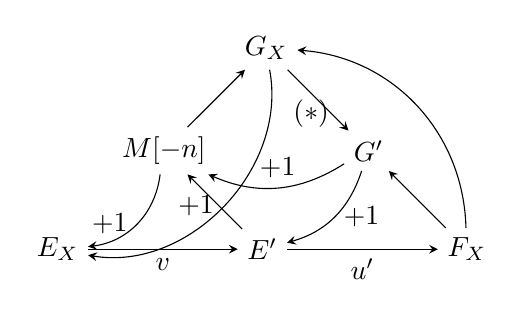
\begin{tikzpicture}[>=stealth,baseline=(GX.base),node distance=1.0cm]
  \node (EX) at (0,0) {$E_X$};
  \node (Ep) at (2.6,0) {$E'$};
  \node (FX) at (5.2,0) {$F_X$};
  \node (M)  at (1.35,1.25) {$M[-n]$};
  \node (GX) at (2.65,2.55) {$G_X$};
  \node (Gp) at (3.95,1.25) {$G'$};
  \node at (3.22,1.72) {$(*)$};
  \draw[->] (EX) -- node[below] {$v$} (Ep);
  \draw[->] (Ep) -- node[below] {$u'$} (FX);
  \draw[->] (Ep) -- (M);
  \draw[->] (M) -- (GX);
  \draw[->] (GX) -- (Gp);
  \draw[->] (FX) -- (Gp);
  \draw[->] (M) to[bend left=38] node[left] {$+1$} (EX);
  \draw[->] (Gp) to[bend left=28] node[above] {$+1$} (M);
  \draw[->] (Gp) to[bend left=28] node[right] {$+1$} (Ep);
  \draw[->] (GX) to[bend left=55] node[left] {$+1$} (EX);
  \draw[->] (FX) to[bend right=42] (GX);
\end{tikzpicture}
\]
La suite exacte de cohomologie du triangle distingué \((*)\) montre que \(\Ho^n(G_X)\longrightarrow \Ho^n(G')\) est un épimorphisme, donc que \(\Ho^n(G')\) est bien de \(\mathcal C_0\)-type fini.

La correction précédente nous ramène donc au cas où \(\Ho^{n+1}(u)\) est un monomorphisme, ce que nous supposerons maintenant. La suite exacte de cohomologie de \(E\to F\to G\) donne alors une suite exacte
\begin{equation}\tag{(.)}
  \Ho^n(E)\xrightarrow{\Ho^n(u)}
  \Ho^n(F)\longrightarrow \Ho^n(G)\longrightarrow 0.
\end{equation}
Comme \(\Ho^n(G)\) est de \(\mathcal C_0\)-type fini, l'ensemble des \(X\) au-dessus de \(S\) tels qu'il existe un épimorphisme \(M\longrightarrow \Ho^n(G_X)\) avec \(M\in\Ob\mathcal C_{0,X}\) est, par définition, un raffinement de \(S\). Utilisant la quasi-relevabilité de \(\mathcal C_0\) dans \(\mathcal C\), on peut imposer que cet épimorphisme se factorise à travers \(Z^n(F_X)\) en
\[
  M\xrightarrow{s}Z^n(F_X)\longrightarrow \Ho^n(F_X)\longrightarrow \Ho^n(G_X).
\]
Il est clair que \(u'\), défini comme en (1.4.1) avec \((r=0)\), est un morphisme de complexes et que \(\Ho^{n+1}(u')=\Ho^{n+1}(u_X)\). D'autre part, il est immédiat, à partir de la suite exacte (.), que
\[
  \Ho^n(u'):\Ho^n(E_X)\oplus M\longrightarrow \Ho^n(F_X)
\]
est un


\medskip\hrule\medskip

% from main.tex
%%%%%%%%%%  scan idx 106  |  folio 93  %%%%%%%%%%
épimorphisme. Cela termine la démonstration de (1.4.1).

\textbf{Lemme 1.4.2.} \emph{Soient \(\mathcal C\) une catégorie abélienne, \(u:E\to F\) un morphisme de complexes de \(\mathcal C\) (resp.\ une flèche de \(\Dpx(\mathcal C)\)), \(G\) le cône de \(u\). Conditions équivalentes pour \(n\in\mathbb Z\) donné} :
\begin{enumerate}[label=(\roman*)]
\item \emph{\(\Ho^i(G)=0\) pour \(i\geq n\)}~;
\item \emph{\(\Ho^i(u)\) est un isomorphisme pour \(i>n\) et un épimorphisme pour \(i=n\)}.
\end{enumerate}
La preuve est immédiate à partir de la suite exacte de cohomologie.

\textbf{Définition 1.4.3.} \emph{Nous dirons que \(u\) est un \(n\)-quasi-isomorphisme (resp.\ un \(n\)-isomorphisme) si \(u\) vérifie les conditions équivalentes de (1.4.2).}

Cela étant, on déduit aussitôt de (1.4.1) le

\textbf{Corollaire 1.4.4.} \emph{Soient \(S,S,\mathcal C,\mathcal C_0\) comme en (1.4.1). Soit \(u:E\to F\) un \((n+1)\)-quasi-isomorphisme de complexes de \(\mathcal C_S\) (\(n\in\mathbb Z\) donné) tel que \(\Ho^n(G)\) soit de \(\mathcal C_0\)-type fini. Alors l'ensemble des \(X\) au-dessus de \(S\) tels qu'il existe \((M,r,s)\) comme en (1.4.1) tels que \(u'\) soit un \(n\)-quasi-isomorphisme est un raffinement de \(S\).}

De manière imagée, on peut, moyennant la condition de finitude sur \(\Ho^n(G)\), localement «~gagner un cran~», i.e. modifier localement \(u\) en degré \(n\) par l'addition à \(E^n\) d'un objet de \(\mathcal C_0\) de manière à faire de \(u\) un \(n\)-quasi-isomorphisme.

\textbf{Corollaire 1.4.5.} Soient \(\mathcal C\) une catégorie abélienne, \(n\in\mathbb Z\), et \(u:E\to F\) un \(n\)-quasi-isomorphisme de complexes de \(\mathcal C\). Il existe un diagramme commutatif de \(\Cpx(\mathcal C)\)
\[
\begin{tikzcd}
E \arrow[r,"v"] \arrow[d,"u"'] & E' \arrow[dl,"u'"]\\
F &
\end{tikzcd}
\]


\medskip\hrule\medskip

% from main.tex
%%%%%%%%%%  scan idx 107  |  folio 94  %%%%%%%%%%
où \(u'\) est un
quasi-isomorphisme et \(v\) un monomorphisme induisant l'identité en degré \(\geq n\) (i.e. tel que \(E'^i=E^i\) et \(v^i=\id(E^i)\) pour \(i\geq n\)).

\emph{Preuve.} Appliquant (1.4.4) dans le cas où \(S\) est le site ponctuel et \(\mathcal C_0=\mathcal C\), on obtient un triangle commutatif de \(\Cpx(\mathcal C)\)
\[
\begin{tikzcd}
E \arrow[r,"v_{n-1}"] \arrow[d,"u"'] & E'_{\,n-1} \arrow[dl,"u'_{n-1}"]\\
F &
\end{tikzcd}
\]
où \(u'_{n-1}\) est un \((n-1)\)-quasi-isomorphisme et \(v_{n-1}\) un monomorphisme induisant l'identité en degré \(\geq n\). Itérant le procédé, on trouve, pour \(i\leq n-1\), une suite de triangles commutatifs de \(\Cpx(\mathcal C)\)
\[
\begin{tikzcd}
E'_i \arrow[r,"v_{i-1}"] \arrow[d,"u'_i"'] & E'_{\,i-1} \arrow[dl,"u'_{i-1}"]\\
F &
\end{tikzcd}
\]
où \(u'_i\) est un \(i\)-quasi-isomorphisme et \(v_{i-1}\) un monomorphisme induisant l'identité en degré \(\geq i\). Le corollaire s'en déduit par passage à la limite. De manière précise, notant \(d'_i\) la différentielle de \(E'_i\), on définit \(E'\) par
\[
  E'^i=E^i,\quad d'^i=d^i\quad\text{pour }i\geq n,
\]
et
\[
  E'^i=(E'_i)^i,\quad d'^i=(d'_i)^i\quad\text{pour }i<n,
\]
puis \(v\) et \(u'\) par
\[
  v^j=(v_i)^j,\qquad u'^j=(u'_i)^j\qquad\text{pour }i\leq j,
\]
et l'on vérifie aussitôt que \(E'\), \(v\), \(u'\) ainsi définis répondent à la question.



\medskip\hrule\medskip

% from main.tex
%%%%%%%%%%  scan idx 108  |  folio 95  %%%%%%%%%%
Autrement dit, en abrégé, on peut prolonger un \(n\)-quasi-isomorphisme en un quasi-isomorphisme «~sans rien changer à ce qui est donné en degré \(\geq n\)~».

\section*{2. Complexes pseudo-cohérents}

\textbf{2.0.} Dans ce numéro, \(S\) désigne un site, \(S\) un objet de \(S\), \(\mathcal C\) une \(S\)-catégorie abélienne plate (1.1), \(\mathcal C_0\) une sous-\(S\)-catégorie additive strictement pleine de \(\mathcal C\). On suppose que \(\mathcal C_0\) est localement quasi-stable par noyau d'épimorphisme (1.2) et localement quasi-relevable dans \(\mathcal C\) (1.2).

\textbf{Définition 2.1.} \emph{Soient \(X\in\Ob S\), \(E\) un complexe de \(\mathcal C_X\), et \(n\in\mathbb Z\). Nous dirons que \(E\) est strictement \(\mathcal C_0\)-\(n\)-pseudo-cohérent (resp.\ \(\mathcal C_0\)-pseudo-cohérent, resp.\ \(\mathcal C_0\)-parfait) si \(E^i=0\) pour \(i\) assez grand et \(E^i\in\Ob\mathcal C_{0,S}\) pour \(i\geq n\) (resp.\ pour tout \(i\), resp.\ pour tout \(i\) et \(E^i=0\) pour presque tout \(i\)).}

Quand il n'y aura pas de confusion à craindre, nous dirons parfois «~strictement \(n\)-pseudo-cohérent (resp\dots)~» au lieu de «~strictement \(\mathcal C_0\)-\(n\)-pseudo-cohérent (resp\dots)~».

\textbf{Lemme 2.1.1.} \emph{Soient \(E\in\Ob\Cpx(\mathcal C_S)\) et \(n\in\mathbb Z\). Si \(E\) est strictement \(n\)-pseudo-cohérent et si \(\Ho^i(E)=0\) pour \(i>n\), alors \(\Ho^n(E)\) est de type fini.}

\emph{Preuve.} La suite
\[
  0\longrightarrow Z^n(E)\longrightarrow E^n\longrightarrow E^{n+1}\longrightarrow\cdots\longrightarrow 0
\]
est exacte et \(E^i\in\Ob\mathcal C_0\) pour \(i\geq n\). Comme \(\mathcal C_0\) est localement quasi-stable par noyau d'épimorphisme, il s'ensuit que \(Z^n(E)\) est de type fini, donc aussi \(\Ho^n(E)\), qui en est un quotient.


\end{document}
